\documentclass[10pt,a4paper]{article}
\usepackage[margin=2.2cm]{geometry}
\usepackage{amsmath,amssymb,amsthm,graphicx,booktabs,caption,float,xcolor,enumitem}
\usepackage{tikz}
\usetikzlibrary{arrows.meta,positioning,fit,calc,shapes.geometric,backgrounds,decorations.pathreplacing}
\usepackage[colorlinks=true,linkcolor=blue!50!black,citecolor=blue!50!black,urlcolor=blue!50!black]{hyperref}
\captionsetup{font=small,labelfont=bf}
\setlist{itemsep=1pt,topsep=3pt}
\graphicspath{{figures/}}
\newcommand{\G}{\mathcal{G}}
\newcommand{\E}{\mathbb{E}}
\newcommand{\Prob}{\mathbb{P}}
\newcommand{\Bin}{\operatorname{Bin}}
\newcommand{\Pool}{\mathcal{P}}
\newcommand{\Win}{\mathcal{W}}
\newcommand{\Fac}{\mathcal{F}}
\newcommand{\U}{\mathcal{U}}
\newcommand{\ind}{\mathbf{1}}
\definecolor{mfour}{HTML}{d1495b}
\definecolor{mthree}{HTML}{3b75af}
\newtheorem{hypothesis}{Hypothesis}

\title{\textbf{Facts as alleles:}\\[2pt] \textbf{a finite-swarm theory of reading, forgetting and persistent influence in swarms of Bayesian agents}}
\author{MA-CC project, task003 LLM-free study (Simulation 2)}
\date{23 October 2026}

\begin{document}
\maketitle

\begin{abstract}
\noindent
A swarm of 24 exact Bayesian agents shares a message board on which a hidden controller posts true but selected facts
to steer the swarm toward a wrong answer. Two phenomena are robust in simulation. \emph{Reading reversal}: reading more
posts per action helps the controller when agents forget fast and protects the swarm when they remember.
\emph{Persistence}: the controller's effect stays almost unchanged long after it stops posting. We ask for the smallest
model that reproduces both, and we judge each candidate on data it was not chosen on. Two deterministic mean-field
models (M1, M2) fail: they get held-out signs at chance and the effect size about three times too small. Diagnostics locate
the cause: each fact is held by only about 1.3 agents, facts go extinct, and extinction carries most of the effect;
a deterministic theory has infinitely many copies of every fact and cannot represent it. Adding integer holder counts
with absorption at zero (M3) recovers most signs but only about 60\% of the magnitude. Adding one shared, realised
board (M4) reproduces held-out effect sizes within 0.03, the ordering and time scales of four post-stop experiments,
the shift of the reversal in worlds made of $K=2$ and $4$ independent copies of the task, and, in a pre-registered
test on a second task (MuSR Object Placements), the effect size within 0.02--0.03 and the main crossover exactly.
The working account is population-genetic: facts behave like alleles, reading is reproduction, forgetting is death,
posting is selection and the controller is immigration.
\end{abstract}

% ======================================================================================================================
\section{Introduction}

Groups of reasoning agents that exchange evidence are increasingly built from language models. Before asking how such
groups can be manipulated, it helps to study a version in which every individual is an \emph{exact} reasoner, so that
any failure is a property of the collective and not of individual reasoning errors. Our simulator does this: each agent
holds a set of true facts about a small logic puzzle, computes the exact Bayesian posterior over the puzzle's answers,
votes, and posts one fact to a shared board; agents forget facts at a constant rate and relearn them by reading the
board. A \emph{false controller} posts true facts, chosen to make a wrong answer look likely.

Earlier analyses of this simulator established two phenomena (Section~\ref{sec:phenomena}):
\begin{itemize}
\item \textbf{Reading reversal.} Let $q$ be the number of posts an agent reads per action and $\rho$ the probability that
  a remembered fact survives one time unit. At small $\rho$, larger $q$ \emph{increases} the controller's effect; at
  large $\rho$ it \emph{decreases} it. The crossover moves with $q$ and with the task.
\item \textbf{Persistence.} After the controller stops, its effect stays nearly constant for at least 100 time units,
  although every agent keeps reading, forgetting and voting.
\end{itemize}

\paragraph{Question.} What is the smallest dynamical model, using the simulator's exact single-agent rules, that
reproduces both phenomena quantitatively on data it was not fitted to?

\paragraph{Contributions.}
\begin{enumerate}
\item A ladder of four models (M1--M4), each adding one ingredient to the previous one (Section~\ref{sec:theory},
  Fig.~\ref{fig:ladder}), with no free parameters: every rate comes from the simulator's rules.
\item A negative result with a diagnosis: deterministic mean-field theories fail, and three diagnostics show that the
  missing ingredient is the \emph{extinction of facts held by very few agents} (Section~\ref{sec:m1m2}).
\item A finite-swarm model (M4) that passes a pre-registered held-out split on the original task, four post-stop
  experiments, a scaling family, and a pre-registered test on a second task (Sections~\ref{sec:m4}--\ref{sec:op}).
\item An interpretation in which facts are alleles of a population-genetic process, which explains why reading can
  both help and hurt (Section~\ref{sec:alleles}).
\end{enumerate}

% ======================================================================================================================
\section{The system}
\label{sec:system}

This section states the simulator's rules as equations. They are not a model: they are extracted from the code
(Simulation~2, continuous time) and every model in Section~\ref{sec:theory} reuses them.

\begin{figure}[t]
\centering
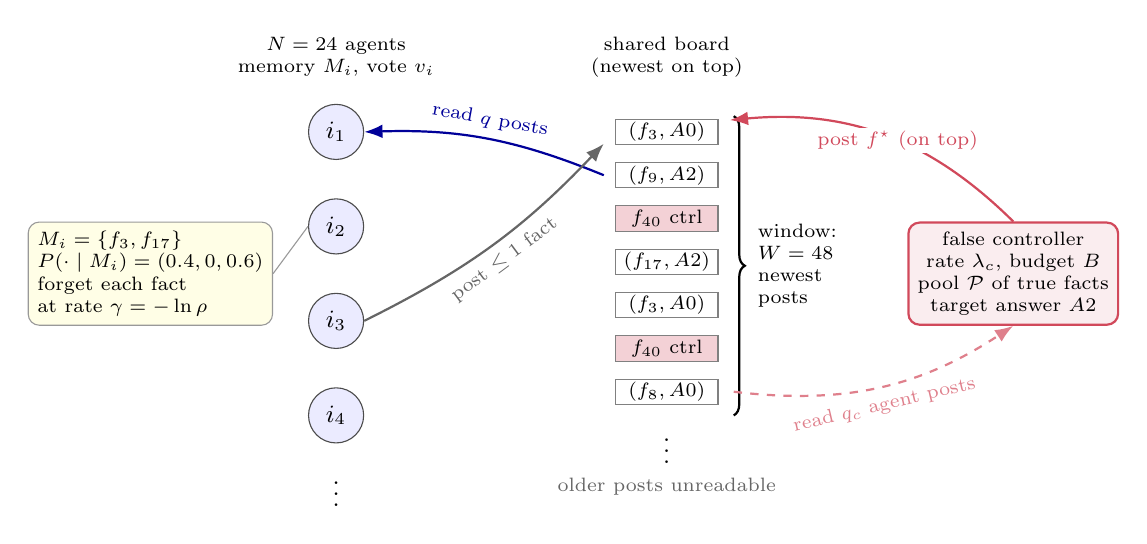
\begin{tikzpicture}[font=\small, >=Latex,
  agent/.style={circle, draw=black!70, fill=blue!8, minimum size=7mm, inner sep=0pt},
  post/.style={rectangle, draw=black!50, fill=white, minimum width=13mm, minimum height=3.2mm, inner sep=0pt, font=\scriptsize},
  cpost/.style={post, fill=mfour!25}]
  % agents
  \foreach \i/\y in {1/2.4,2/1.2,3/0,4/-1.2} {\node[agent] (a\i) at (0,\y) {$i_{\i}$};}
  \node at (0,-2.1) {$\vdots$};
  \node[align=center, font=\scriptsize] at (0,3.35) {$N=24$ agents\\memory $M_i$, vote $v_i$};
  \node[draw=black!40, rounded corners, fill=yellow!10, font=\scriptsize, align=left, anchor=east] (mem) at (-0.8,0.6)
    {$M_i=\{f_3,f_{17}\}$\\$P(\cdot\mid M_i)=(0.4,0,0.6)$\\forget each fact\\at rate $\gamma=-\ln\rho$};
  \draw[black!40] (mem.east) -- (a2.west);
  % board
  \begin{scope}[shift={(4.2,0)}]
    \foreach \k/\t in {0/{$(f_3,A0)$},1/{$(f_9,A2)$},2/{$f_{40}$ ctrl},3/{$(f_{17},A2)$},4/{$(f_3,A0)$},5/{$f_{40}$ ctrl},6/{$(f_8,A0)$}} {
      \pgfmathsetmacro{\yy}{2.4-0.55*\k}
      \ifnum\k=2 \node[cpost] at (0,\yy) {\t}; \else \ifnum\k=5 \node[cpost] at (0,\yy) {\t}; \else \node[post] at (0,\yy) {\t}; \fi\fi
    }
    \node at (0,-1.55) {$\vdots$};
    \draw[decorate, decoration={brace, amplitude=4pt}, thick] (0.85,2.6) -- (0.85,-1.2) node[midway, right=5pt, font=\scriptsize, align=left] {window:\\$W=48$\\newest\\posts};
    \node[align=center, font=\scriptsize] at (0,3.35) {shared board\\(newest on top)};
    \node[font=\scriptsize, black!60] at (0,-2.1) {older posts unreadable};
  \end{scope}
  % controller
  \node[draw=mfour, thick, fill=mfour!10, rounded corners, align=center, font=\scriptsize] (c) at (8.6,0.6)
     {false controller\\rate $\lambda_c$, budget $B$\\pool $\Pool$ of true facts\\target answer $A2$};
  % arrows
  \draw[->, thick, blue!60!black] (3.4,1.85) to[bend right=12] node[above, font=\scriptsize, sloped] {read $q$ posts} (a1.east);
  \draw[->, thick, black!60] (a3.east) to[bend right=10] node[below, font=\scriptsize, sloped] {post $\le 1$ fact} (3.4,2.25);
  \draw[->, thick, mfour] (c.north) to[bend right=25] node[font=\scriptsize, pos=0.45, fill=white, inner sep=1pt] {post $f^\star$ (on top)} (5.0,2.55);
  \draw[->, thick, mfour!70, dashed] (5.05,-0.9) to[bend right=20] node[below, font=\scriptsize, sloped] {read $q_c$ agent posts} (c.south);
\end{tikzpicture}
\caption{\textbf{The system.} Each agent holds a memory $M_i$ of true facts, computes the exact posterior over the three
answers, votes, and posts one fact that supports its vote. Every action begins by reading $q$ posts from the $W$ newest
posts of others. Facts are forgotten at rate $\gamma=-\ln\rho$. A false controller (red) reads agents' posts and posts the
pool fact that most raises the probability of the wrong answer $A2$; it stops at $t_c=30$ or when its budget is spent.}
\label{fig:system}
\end{figure}

\subsection{World and beliefs}
A \emph{world} is a finite set $\Omega$ of possible states (complete assignments of the puzzle's hidden quantities) with
weights $\pi(\omega)>0$, partitioned by the answer each state implies: $\Omega=\Omega_{A0}\cup\Omega_{A1}\cup\Omega_{A2}$.
A \emph{fact} $f$ is a true statement, identified with the set $\Omega_f\subseteq\Omega$ of states consistent with it.
For a set of facts $M$, let $\Omega(M)=\bigcap_{f\in M}\Omega_f$ (with $\Omega(\emptyset)=\Omega$). The exact posterior
of an agent who remembers $M$ is
\begin{equation}
  P(a\mid M)\;=\;\frac{\sum_{\omega\in\Omega_a\cap\Omega(M)}\pi(\omega)}{\sum_{\omega\in\Omega(M)}\pi(\omega)},
  \qquad a\in\{A0,A1,A2\}.
  \label{eq:posterior}
\end{equation}
In task003 (Section~\ref{sec:tasks}) $\pi$ is uniform over 14{,}388 states; in Object Placements it is the generator's
probability of each of 617{,}472 stories. Facts combine by intersection, not additively: a set $M$ can \emph{prove} an
answer ($P(a\mid M)=1$) although no member does.

\subsection{Agents}
There are $N=24$ agents. Agent $i$ starts with one fact, $M_i(0)=\{f_i^0\}$. It acts at the events of a Poisson clock
of rate $\lambda_a=1$. At an action at time $t$:
\begin{enumerate}[label=(\roman*)]
\item \textbf{Read.} Let $\Win_i(t)$ be the $W=48$ newest posts on the board not authored by $i$. The agent draws a set
  $S$ of $\min(q,|\Win_i(t)|)$ posts uniformly without replacement and adds their facts $\Fac(S)$ to memory:
  \begin{equation}
    M_i\;\leftarrow\;M_i\cup\Fac(S).\label{eq:read}
  \end{equation}
  A fact carried by $k$ of the $W$ posts is read with probability $1-\binom{W-k}{q}\big/\binom{W}{q}$: exposure grows with
  the number of \emph{copies} of a fact on the board.
\item \textbf{Vote.} The vote is drawn from the posterior (probability matching):
  \begin{equation}
    v_i\sim P(\cdot\mid M_i).\label{eq:vote}
  \end{equation}
\item \textbf{Post.} The agent posts one fact that supports its vote \emph{in the context of its memory}. The candidates
  are
  \begin{equation}
    C(M,v)=\{f\in M:\;P(v\mid M)>P(v\mid M\setminus\{f\})\},\label{eq:candidates}
  \end{equation}
  facts whose removal would lower the belief in $v$. If $C$ is empty, the fallback is $\{f\in M: P(v\mid\{f\})>1/3\}$;
  if that is empty, nothing is posted. If some candidates were not just read, only those are kept. One candidate is
  chosen uniformly; the post records the pair (fact, author's vote).
\end{enumerate}
\textbf{Forgetting.} Each remembered fact has an independent exponential lifetime of rate
\begin{equation}
  \gamma=-\ln\rho,\label{eq:gamma}
\end{equation}
so $\rho$ is the probability that a fact survives one time unit; rereading a fact restarts its lifetime; the starting
fact is forgettable; $\rho=1$ means no forgetting.

\subsection{Controller}
The false controller targets $a^\star=A2$. It acts at rate $\lambda_c=1$ for $t<t_c=30$ while fewer than $B=30$ posts
have been made. At an action it reads $q_c=12$ of the $W$ newest \emph{agent} posts, giving facts $R$ and the share
$\hat v$ of those posts whose author voted $a^\star$. It stays silent if $\hat v\ge\theta=0.75$ (the \emph{gate}).
Otherwise it posts
\begin{equation}
  f^\star(R)=\arg\max_{f\in\Pool}P(a^\star\mid R\cup\{f\}),\label{eq:controller}
\end{equation}
where $\Pool$ is its pool of 12 true facts (ties broken by fact identifier; if the maximum is 0, $P(a^\star\mid\{f\})$
is maximised instead). The rule is deterministic given $R$.

\subsection{Observables}
Let $x_a(t)$ be the share of vote $a$ among agents who have voted at least once. Every run is \emph{paired}: an episode
$e$ is simulated in a \emph{false} arm (controller active) and a \emph{silent} arm (no controller) with identical random
streams (all keyed by seed, episode and purpose, never by arm or setting). The \textbf{controller effect} is
\begin{equation}
  G(\rho,q)=\E_e\!\left[x_{A2}^{\text{false}}(30)-x_{A2}^{\text{silent}}(30)\right],\label{eq:G}
\end{equation}
the \textbf{reading increment} is
\begin{equation}
  D(q_1\!\to\!q_2;\rho)=G(\rho,q_2)-G(\rho,q_1),\label{eq:D}
\end{equation}
estimated per episode (streams are shared across $q$ too), and after the controller stops
\begin{equation}
  \delta(t)=\E_e\!\left[x_{A2}^{\text{false}}(t)-x_{A2}^{\text{silent}}(t)\right],\qquad t\ge t_c .\label{eq:delta}
\end{equation}
Persistence experiments continue the system after $t_c$ in four modes: \emph{normal}; \emph{no communication} (no
reading, no posting); \emph{frozen board} (agents read only the board as it was at $t_c$, nobody posts); \emph{controller
facts removed} (facts only the controller had are deleted from memories and board, then normal). A data increment is
\emph{resolved} when its 95\% interval excludes 0.

\subsection{Tasks and setups}
\label{sec:tasks}
\textbf{task003} (team allocation): 3 people, 2 jobs, 3 candidate allocations; 49 true facts; $A0$ is correct, $A2$ is the
controller's target. Two frozen setups: \emph{symmetric}, in which the 24 agents' 18 distinct facts jointly prove $A0$ but
no single fact or pair does; and \emph{no-proof}, in which the agents' 15 distinct facts leave $(0.5,0,0.5)$ and nothing
can be proved. \textbf{K projects} (Section~\ref{sec:scaling}): $K$ independent copies of task003 answered by one split,
with $24K$ agents, $W$, $\lambda_c$ and $B$ multiplied by $K$. \textbf{Object Placements} (Section~\ref{sec:op}): a story
from the MuSR benchmark~\cite{sprague2024musr}, rebuilt exactly with the same setup rules.

% ======================================================================================================================
\section{Theory: four reduced models}
\label{sec:theory}

\subsection{Common representation}
All four models replace the $N$-agent swarm by a \emph{population} of $\mathcal{K}=NR$ agents ($R$ copies of every agent
of the setup) and advance time in steps of $dt=0.05$. Every population agent applies Eqs.~\eqref{eq:posterior}--\eqref{eq:candidates}
exactly, using the simulator's own code. In one step:
\begin{itemize}
\item each remembered fact is forgotten with probability $1-\rho^{dt}$ (exact for exponential lifetimes as
  $dt\to0$, since they are memoryless);
\item each agent acts with probability $\lambda_a dt$; an acting agent reads, votes and posts as in
  Eqs.~\eqref{eq:read}--\eqref{eq:candidates}.
\end{itemize}
Votes are kept per agent, so the lag between belief and vote is exact. The models differ only in \emph{what agents read}
and \emph{how facts are counted}. Table~\ref{tab:notation} lists the notation.

\begin{table}[h]
\centering\small
\begin{tabular}{@{}ll@{}}
\toprule
symbol & meaning \\
\midrule
$N$, $\mathcal{K}=NR$, $R$ & swarm size (24), population size, number of population copies of the swarm \\
$\U$ & circulating facts: agents' starting facts $\cup$ controller-only pool facts \\
$c=(f,v)$ or $c=(f,\text{ctrl})$ & post category: fact $f$ posted by an agent who voted $v$, or by the controller \\
$h(t)\in\mathbb{R}_{\ge0}^{|\mathcal{C}|}$ & posts entering the board during step $t$, per category (in swarm units) \\
$b(t)$ & expected composition of the $W$ newest posts (M1--M3) \\
$\mathcal{B}(t)$ & realised board: an ordered list of posts (M4) \\
$H_f(t)$, $m_f(t)=H_f/\mathcal{K}$ & number and share of population agents holding fact $f$ \\
$n_f(t)\in\{0,\dots,N\}$ & integer number of holders of $f$ in the swarm (M3, M4) \\
$\ell_f(t)$, $g_f(t)$ & per-step probability that a holder loses $f$, that a non-holder gains $f$ \\
$\mathrm{copies}_f$ & number of copies of $f$ among the $W$ newest posts \\
$u_f(t)$ & expected controller posts of $f$ in step $t$ (M1--M3) \\
\bottomrule
\end{tabular}
\caption{Notation of the reduced models (in addition to Section~\ref{sec:system}).}
\label{tab:notation}
\end{table}

\begin{figure}[t]
\centering
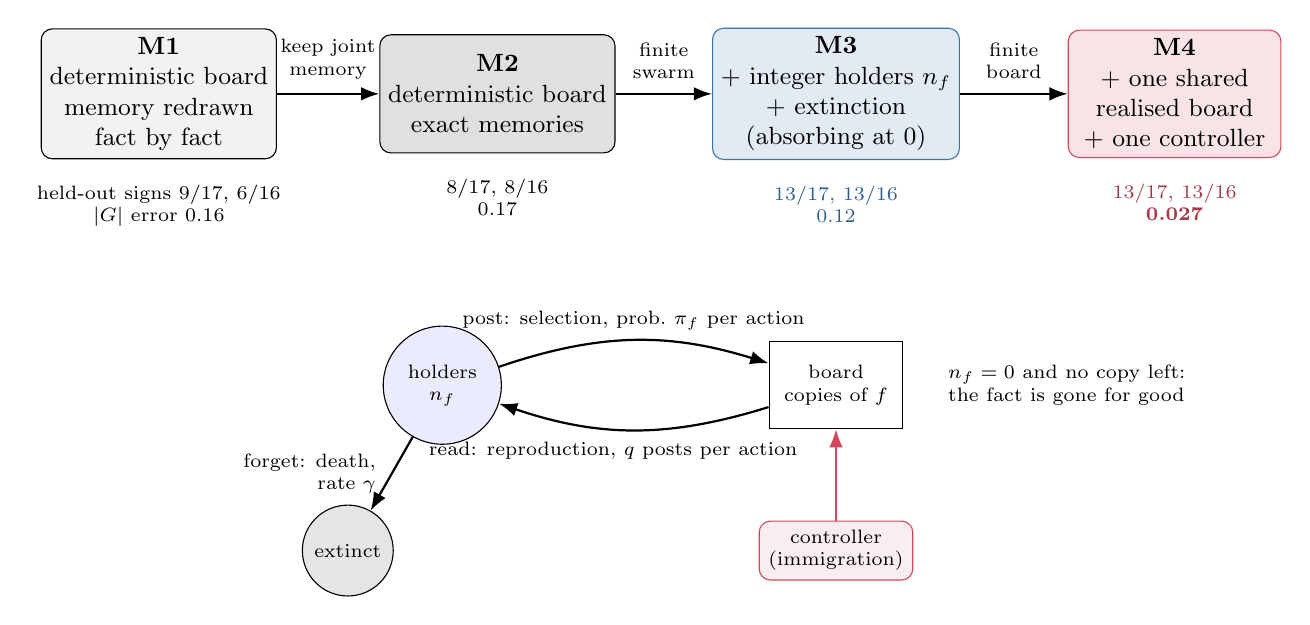
\begin{tikzpicture}[font=\small, >=Latex,
  box/.style={draw, rounded corners, align=center, minimum width=27mm, minimum height=15mm, inner sep=3pt},
  add/.style={font=\scriptsize, align=center, inner sep=1pt}]
  \node[box, fill=black!5]  (m1) at (0,0) {\textbf{M1}\\deterministic board\\memory redrawn\\fact by fact};
  \node[box, fill=black!12] (m2) at (4.3,0) {\textbf{M2}\\deterministic board\\exact memories};
  \node[box, fill=mthree!15, draw=mthree] (m3) at (8.6,0) {\textbf{M3}\\+ integer holders $n_f$\\+ extinction\\(absorbing at 0)};
  \node[box, fill=mfour!15, draw=mfour] (m4) at (12.9,0) {\textbf{M4}\\+ one shared\\realised board\\+ one controller};
  \draw[->, thick] (m1) -- node[add, above=4pt] {keep joint\\memory} (m2);
  \draw[->, thick] (m2) -- node[add, above=4pt] {finite\\swarm} (m3);
  \draw[->, thick] (m3) -- node[add, above=4pt] {finite\\board} (m4);
  \node[font=\scriptsize, align=center, below=2mm of m1] {held-out signs 9/17, 6/16\\$|G|$ error 0.16};
  \node[font=\scriptsize, align=center, below=2mm of m2] {8/17, 8/16\\0.17};
  \node[font=\scriptsize, align=center, below=2mm of m3, mthree!80!black] {13/17, 13/16\\0.12};
  \node[font=\scriptsize, align=center, below=2mm of m4, mfour!80!black] {13/17, 13/16\\\textbf{0.027}};
  % allele cycle
  \begin{scope}[shift={(3.6,-3.7)}]
    \node[draw, circle, fill=blue!8, minimum size=15mm, align=center, font=\scriptsize] (H) at (0,0) {holders\\$n_f$};
    \node[draw, rectangle, fill=white, minimum width=17mm, minimum height=11mm, align=center, font=\scriptsize] (Bf) at (5,0) {board\\copies of $f$};
    \node[draw, circle, fill=black!10, minimum size=10mm, font=\scriptsize] (X) at (-1.2,-2.1) {extinct};
    \node[draw=mfour, rounded corners, fill=mfour!10, font=\scriptsize, align=center] (C) at (5,-2.1) {controller\\(immigration)};
    \draw[->, thick] (H) to[bend left=18] node[above, font=\scriptsize] {post: selection, prob.\ $\pi_f$ per action} (Bf);
    \draw[->, thick] (Bf) to[bend left=18] node[below=1pt, font=\scriptsize, pos=0.58] {read: reproduction, $q$ posts per action} (H);
    \draw[->, thick] (H) -- node[left=2pt, font=\scriptsize, align=right] {forget: death,\\rate $\gamma$} (X);
    \draw[->, thick, mfour] (C) -- (Bf);
    \node[font=\scriptsize, align=left, anchor=west] at (6.3,0) {$n_f=0$ and no copy left:\\the fact is gone for good};
  \end{scope}
\end{tikzpicture}
\caption{\textbf{Top: the model ladder.} Each model adds one ingredient to the previous one; below each box, the
pre-registered held-out score on task003 (resolved signs of $D$ right, symmetric and no-proof; mean $|G|$ error).
\textbf{Bottom: the allele picture} (Section~\ref{sec:alleles}). A fact reproduces when a post of it is read by a
non-holder, dies when forgotten, is selected by the posting rule, and immigrates from the controller. With about 1.3
holders per fact, drift drives facts extinct, and extinction is permanent.}
\label{fig:ladder}
\end{figure}

\subsection{M2: deterministic mean field with exact memories}
The board is \emph{deterministic}: it is the expected composition of the posts of the swarm. Population posts are
rescaled to the swarm's posting rate, and the controller contributes its expected posts:
\begin{equation}
  h_c(t)=\frac{1}{R}\sum_{i=1}^{\mathcal{K}}\ind[\,i\text{ acts and posts category }c\text{ in step }t\,]
        \;+\;u_f(t)\,\ind[c=(f,\text{ctrl})].\label{eq:h}
\end{equation}
The readable board $b(t)$ is the newest $W$ posts of this history: with $h^{(k)}=h(t-k\,dt)$,
\begin{equation}
  b(t)=\sum_{k\ge0}w_k\,h^{(k)},\qquad
  w_k=\min\!\Big(1,\max\!\Big(0,\tfrac{W-\sum_{j<k}|h^{(j)}|}{|h^{(k)}|}\Big)\Big),\label{eq:window}
\end{equation}
where $|h|$ is the total number of posts in $h$. The controller is replaced by its expected posting:
\begin{equation}
  u_f(t)=\lambda_c\,dt\;\Prob_{R\sim b^{\text{ag}}(t)}\!\big[\hat v<\theta\ \text{and}\ f^\star(R)=f\big],\label{eq:u}
\end{equation}
estimated by drawing $q_c$ posts 60 times from the agent-post part $b^{\text{ag}}$ of the board and applying
Eq.~\eqref{eq:controller}; its total is capped by the remaining budget. A reader draws its own realisation of the board
and then $q$ posts from it:
\begin{equation}
  \tilde B_i\sim\mathrm{Multinomial}\big(\lfloor|b|\rceil,\;b/|b|\big),\qquad S_i\sim\mathrm{Hypergeometric}(\tilde B_i,q).\label{eq:mfread}
\end{equation}
Each agent keeps its exact memory set $M_i$, so the joint structure of an agent's evidence, such as the several facts
that together prove $A0$, is kept. Correlations \emph{between} agents and all finite-size effects are dropped: with
$\mathcal{K}\to\infty$, every fact has infinitely many holders.

\subsection{M1: fact-by-fact closure}
M1 is M2 with one change: before each action an agent's memory is redrawn independently fact by fact from the
population shares,
\begin{equation}
  M_i\leftarrow\{f\in\U:\ \xi_{if}<m_f(t)\},\qquad \xi_{if}\overset{\text{iid}}{\sim}\mathrm{Uniform}(0,1).\label{eq:m1}
\end{equation}
This removes all joint structure in memory: the memory distribution becomes a product of independent per-fact
Bernoulli variables with means $m_f$, the closure behind a rate equation for the shares $m_f$.

\subsection{M3: finite-swarm holder counts and extinction}
M3 keeps M2's population and board, and adds an integer number of holders $n_f$ of every circulating fact in a swarm
of $N$ agents, initialised to the setup's holders (1 or 2). In each step, the population's deterministic step gives
per-fact loss and gain probabilities, measured on the memories before ($M^-$) and after ($M^+$) the step:
\begin{equation}
  \ell_f=\frac{|\{i: f\in M_i^-,\ f\notin M_i^+\}|}{H_f^-},\qquad
  g_f=\frac{|\{i: f\notin M_i^-,\ f\in M_i^+\}|}{\mathcal{K}-H_f^-}.\label{eq:lossgain}
\end{equation}
The swarm counts then change by binomial draws (demographic noise),
\begin{equation}
  n_f(t+dt)=n_f(t)-\Bin\!\big(n_f(t),\ell_f\big)+\Bin\!\big(N-n_f(t),g_f\big),\label{eq:m3}
\end{equation}
and the population is projected onto the new count: holders of $f$ are removed or added at random until
$H_f=\lfloor n_f\mathcal{K}/N\rceil$. \textbf{Extinction} is absorbing:
\begin{equation}
\begin{aligned}
  &n_f=0\ \wedge\ \mathrm{copies}_f(b)<\tfrac12\ \wedge\ \neg\big(\text{controller active}\wedge f\in\Pool\big)\\
  &\qquad\Longrightarrow\; f\text{ is removed from memories and board for good}.
\end{aligned}\label{eq:extinct}
\end{equation}
This is the only finite-swarm ingredient of M3.

\subsection{M4: one shared, realised board}
M4 keeps M3's holder counts and extinction rule and replaces the deterministic board by one \emph{realised} board
$\mathcal{B}(t)$, an ordered list of posts that every population agent reads. Readers draw $q$ posts uniformly without
replacement from the $W$ newest entries of $\mathcal{B}$. In each step, every population post enters $\mathcal{B}$
independently with probability $1/R$, in random order, so the board receives the swarm's posting stream:
\begin{equation}
  \#\{\text{posts of category }c\text{ entering }\mathcal{B}\}\sim\Bin\!\Big(\textstyle\sum_i\ind[i\text{ posts }c],\ \tfrac1R\Big).\label{eq:thin}
\end{equation}
The expected controller of Eq.~\eqref{eq:u} is replaced by \emph{one} stochastic controller that acts with probability
$\lambda_c dt$ per step and applies Eq.~\eqref{eq:controller} to $q_c$ agent posts drawn from $\mathcal{B}$. In
Eq.~\eqref{eq:extinct}, $\mathrm{copies}_f$ is counted on the $W$ newest entries of $\mathcal{B}$. The new
ingredient is a \emph{correlation}: all readers see the same fluctuating board, so a run of controller posts, or the
disappearance of the last copy of an agent fact, reaches the whole swarm at once.

\paragraph{What M4 is and is not.} M4 keeps the exact single-agent rules, a mean-field population for memories, a finite
realised board, and integer holder counts. It drops between-agent correlations other than those through the shared
board. A reader's own posts are not excluded from its window (they are about 1/24 of it). M4 is a reduced
\emph{stochastic} model, not a closed-form theory.

\subsection{The allele picture}
\label{sec:alleles}
M3 and M4 suggest a population-genetic reading (Fig.~\ref{fig:ladder}, bottom). Board posts are copies of facts.
Reading is reproduction: a post read by a non-holder creates a holder. Forgetting is death. The posting rule of
Eq.~\eqref{eq:candidates} is selection, since agents post facts that support their vote. The controller is immigration
of facts that favour $A2$. A heuristic reproduction number follows from three rates:
\begin{itemize}
\item a holder posts $f$ with probability $\pi_f$ per action, and so $\pi_f/\gamma$ times per holding period;
\item posts enter the board at rate $Np_{\text{post}}$, where $p_{\text{post}}$ is the share of actions that post, so a
  post stays readable for $W/(Np_{\text{post}})$ time units;
\item the $W$ posts in the window receive $Nq$ reads per unit time between them.
\end{itemize}
Each post is therefore read $q/p_{\text{post}}$ times, and
\begin{equation}
  \mathcal{R}_f\;\approx\;\frac{\pi_f}{\gamma}\cdot\frac{q}{p_{\text{post}}}\cdot\big(1-m_f\big).\label{eq:Rf}
\end{equation}
A rare fact with $\mathcal{R}_f<1$ dies out; with about 1.3 holders at the start, even $\mathcal{R}_f$ slightly above 1
leaves a large extinction probability~\cite{harris1963}. Eq.~\eqref{eq:Rf} makes the two effects of reading explicit:
larger $q$ raises the reproduction of \emph{every} fact, the controller's included. Small $\gamma$ (good memory) is what
lets agent facts cross the threshold. We state the resulting account as a hypothesis; Section~\ref{sec:results} tests
its consequences through M3 and M4, not Eq.~\eqref{eq:Rf} itself.

\begin{hypothesis}[reading reversal]
At high forgetting rates $\gamma$, agent facts go extinct whatever $q$, so reading more mainly spreads the controller's
facts and amplifies its effect. At low $\gamma$, reading more lifts agent facts above the extinction threshold, lets
the swarm reassemble its joint evidence, and protects it.
\end{hypothesis}
\begin{hypothesis}[persistence]
After the controller stops, its facts become ordinary alleles, and agent facts that went extinct cannot return. The
swarm's composition then changes only by drift and weak selection, so the controller's imprint persists.
\end{hypothesis}

% ======================================================================================================================
\section{Evaluation protocol}
\label{sec:protocol}
\textbf{Pre-registered split.} Before any model was run, task003 cells were split into \emph{development} cells
($\rho\in\{0.25,0.75,1\}$, $q\in\{3,6\}$, $t\le30$) and \emph{held-out} cells (all other $\rho\in\{0.125,\dots,1\}$,
$q\in\{3,6,9,12\}$, and all post-stop data). Model choices could use development data only; each version was scored once on
held-out data. These data had appeared in earlier descriptive reports, so the split constrains model choice, not
exposure. \textbf{Object Placements} predictions of M3 and M4 were committed to the repository before the simulation
data were opened. \textbf{K-projects} scores are post-hoc (data seen first); no model setting was changed for them.

\textbf{Scores.} (i) \emph{Sign}: for every resolved data increment $D$, the model is right if its own increment has the
same sign with $|D_{\text{model}}|\ge0.01$ (smaller is called zero). (ii) \emph{Size}: mean absolute error of $G$.
(iii) \emph{Crossover}: the $\rho$ bracket in which the sign of $D$ changes. (iv) \emph{Persistence}: $\delta(t)$ at
$t=30,31,40,80,130$, the half-time of the no-communication decay, the sign of the residual after removal, and the
ordering of the four modes at $t=40$ and $130$.

\textbf{Numerics.} Simulation: 1{,}000 paired episodes per cell (500 for $K=4$). Models: $dt=0.05$; M1/M2 with $R=100$;
M3/M4 with 40 realisations and $R=30$ on task003, 20 realisations and $R=20$ on Object Placements, and 20 realisations
and $R=10$ on the K worlds. For M2, $G$ changes by at most about 0.02 between $R=50,100,200$ and between $dt=0.05$ and
$0.025$.

% ======================================================================================================================
\section{Results}
\label{sec:results}

\subsection{The phenomena in the simulation}
\label{sec:phenomena}
\begin{figure}[t]
\centering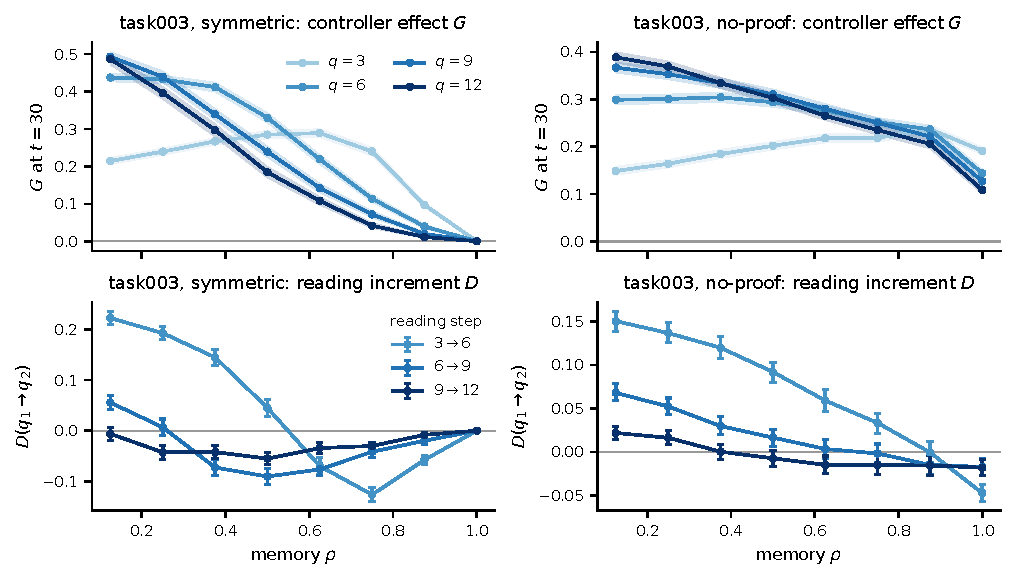
\includegraphics[width=\linewidth]{fig3_task003_data.pdf}
\caption{\textbf{The reading reversal in task003} (simulation, 1{,}000 paired episodes per point, 95\% bands/intervals).
Top: controller effect $G$ (Eq.~\ref{eq:G}) against memory $\rho$ for four reading depths $q$. Bottom: reading increments
$D$ (Eq.~\ref{eq:D}). Positive $D$: reading more helps the controller; negative: reading more protects the swarm. The sign
changes at a $\rho$ that falls as $q$ grows; in the no-proof setup it changes at higher memory.}
\label{fig:data}
\end{figure}
Figure~\ref{fig:data} shows the reversal. In the symmetric setup, $D(3\to6)$ falls from $+0.22$ at $\rho=0.125$ to
$-0.13$ at $\rho=0.75$, changing sign between $\rho=0.5$ and $0.625$. In the no-proof setup it falls from $+0.15$ to
$-0.05$ at $\rho=1$, changing sign between $0.75$ and $1$. The crossover falls with $q$ (symmetric $6\to9$:
$0.125$--$0.375$). At $\rho=1$ the symmetric swarm always assembles its proof and $G=0$. Persistence is shown with the
models in Fig.~\ref{fig:poststop}: under normal continuation and with a frozen board, $\delta(t)$ stays flat to $t=130$;
without communication it vanishes within 1--6 time units; when controller-only facts are removed, it collapses to a
small residual.

\subsection{Deterministic mean field fails, and why}
\label{sec:m1m2}
Both deterministic models fail the pre-registered scorecard (Fig.~\ref{fig:ladder}, top; Fig.~\ref{fig:models}, dashed).
M1 gets 9/17 (symmetric) and 6/16 (no-proof) held-out signs right; M2 gets 8/17 and 8/16, both at chance. Both
underestimate $G$ about threefold (mean errors 0.15--0.18). Three diagnostics locate the cause (Fig.~\ref{fig:diag}):
\begin{enumerate}
\item \textbf{Not an implementation error.} The same code with a real 24-agent board and one stochastic controller
  reproduces the simulator: $G=0.322\pm0.017$ against $0.33$ (symmetric) and $0.288\pm0.013$ against $0.29$ (no-proof) at
  $\rho=0.5$, $q=6$.
\item \textbf{Not the memory closure.} M1 (no joint memory) and M2 (exact joint memory) fail alike.
\item \textbf{Copies per fact.} Replicating the swarm $R$ times, with $W$, $\lambda_c$ and $B$ also multiplied by $R$,
  drives $G$ down to the mean-field value (Fig.~\ref{fig:diag}a). This multiplies agents but not facts, so it raises the
  number of holders per fact ($\approx1.3R$). The series measures redundancy, not swarm size.
\item \textbf{Extinction carries the effect.} Forbidding agents to forget their own starting fact, so that no agent fact
  can vanish, cuts $G$ from 0.44 to 0.09 (symmetric, $\rho=0.25$) and from 0.30 to 0.20 (no-proof)
  (Fig.~\ref{fig:diag}b). This also gives every agent one permanent fact, so it is not a pure switch.
\end{enumerate}
\begin{figure}[t]
\centering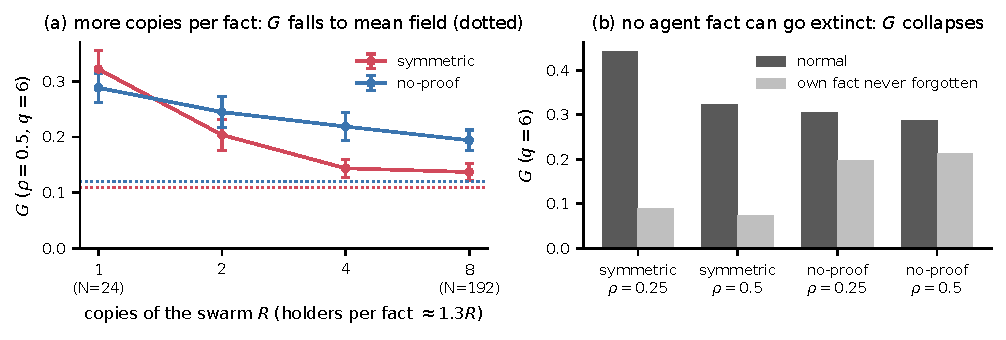
\includegraphics[width=\linewidth]{fig4_diagnostics.pdf}
\caption{\textbf{Why deterministic mean field fails.} (a) The finite-board model at $\rho=0.5$, $q=6$, with the swarm
copied $R$ times (and $W$, $\lambda_c$, $B$ scaled with it): $G$ falls toward the mean-field value (dotted) as each fact
gets more holders (95\% intervals; 300, 200, 120 and 60 paired episodes for $R=1,2,4,8$). (b) When agents never forget their own starting fact,
no agent fact can go extinct, and most of $G$ disappears (300 paired episodes per bar).}
\label{fig:diag}
\end{figure}
A deterministic theory has infinitely many copies of every fact and cannot represent extinction. A system-size expansion
(Gaussian fluctuations of order $1/\sqrt{\mathcal{K}}$~\cite{vankampen1992}) would not help either: the relevant small
parameter is $1/(\text{copies per fact})\approx0.75$, and extinction is an absorbing event, not a small fluctuation.

\subsection{M3: extinction recovers the signs, not the size}
Adding integer holder counts and absorption (Eqs.~\ref{eq:lossgain}--\ref{eq:extinct}) raises held-out signs to 13/17
and 13/16 and lowers the $G$ error to 0.12 (Fig.~\ref{fig:models}, blue). It reproduces the post-stop mechanisms and the
no-communication half-times (1.0, 2.5 and 1.0 time units exactly, 7.5 against 5.5 in the fourth cell). Its magnitudes are
about 60\% of the data. It misses the amplifying side of the symmetric reversal (1 of 4 positive increments right), and
under normal continuation it relaxes by 20--26\% where the data stay flat. The sign of the residual after removal is
right in 2 of 4 cells.

\subsection{M4: a shared finite board closes most of the gap}
\label{sec:m4}
\begin{figure}[t]
\centering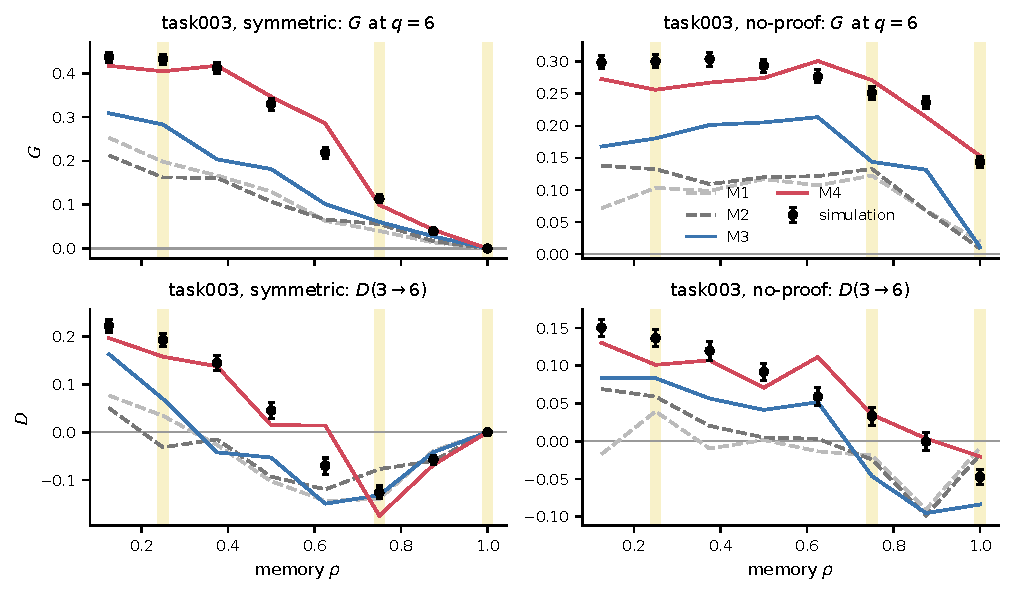
\includegraphics[width=\linewidth]{fig5_models_task003.pdf}
\caption{\textbf{The four models against task003.} Points: simulation (95\% intervals). Lines: models (M1, M2 dashed).
Yellow bands mark the development values of $\rho$; all other points are held out. Top: $G$ at $q=6$. Bottom: $D(3\to6)$.}
\label{fig:models}
\end{figure}
M4 was selected on development data (development $G$ error 0.017, against 0.069 for M3) and then scored once
(Table~\ref{tab:heldout}). On held-out cells its $G$ error is 0.027, a fourfold reduction from M3; it gets all four positive
symmetric increments right, the side M3 missed. All seven held-out misses are at or next to a crossover:
\begin{itemize}
\item symmetric $0.625$ ($3\to6$), $0.875$ ($6\to9$), $0.5$ and $0.875$ ($9\to12$);
\item no-proof $0.375$, $0.875$ and $1$ ($6\to9$).
\end{itemize}
The predicted crossover of $D(3\to6)$ is one step too high in symmetric ($0.625$--$0.75$ against $0.5$--$0.625$) and
exact in no-proof ($0.75$--$1$).

\begin{table}[h]
\centering\small
\resizebox{\linewidth}{!}{%
\begin{tabular}{@{}lcccc@{}}
\toprule
 & M1 & M2 & M3 & M4 \\
\midrule
held-out signs, symmetric (data $+$ / data $-$) & 9/17 (1/4, 8/13) & 8/17 (1/4, 7/13) & 13/17 (1/4, 12/13) & 13/17 (\textbf{4/4}, 9/13) \\
held-out signs, no-proof (data $+$ / data $-$) & 6/16 (2/10, 4/6) & 8/16 (4/10, 4/6) & 13/16 (8/10, 5/6) & 13/16 (9/10, 4/6) \\
held-out $G$ error, symmetric / no-proof & 0.145 / 0.181 & 0.151 / 0.179 & 0.122 / 0.119 & \textbf{0.027 / 0.026} \\
crossover $3\to6$ symmetric (data 0.5--0.625) & 0.25--0.375 & 0.125--0.25 & 0.25--0.375 & 0.625--0.75 \\
crossover $3\to6$ no-proof (data 0.75--1) & two changes & 0.375--0.75 & 0.625--0.75 & \textbf{0.75--1} \\
post-stop ordering ($t=40,130$; 8 cases) & -- & -- & 3/8 & \textbf{7/8} \\
\bottomrule
\end{tabular}}
\caption{Pre-registered held-out scores on task003. Each version was evaluated once.}
\label{tab:heldout}
\end{table}

\begin{figure}[t]
\centering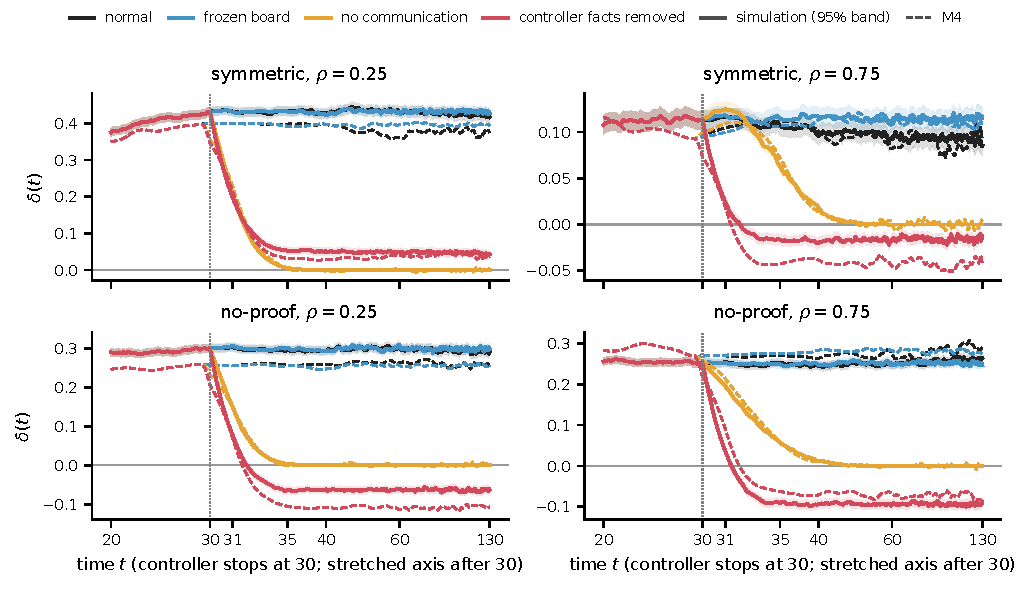
\includegraphics[width=\linewidth]{fig6_post_stop.pdf}
\caption{\textbf{Persistence after the controller stops} ($q=6$; all post-stop data are held out). Solid: simulation
$\delta(t)$ (Eq.~\ref{eq:delta}, 1{,}000 paired episodes, 95\% band). Dashed: M4 (40 realisations, smoothed over 2 time
units). The time axis is stretched after $t_c=30$.}
\label{fig:poststop}
\end{figure}
\textbf{Persistence} (Fig.~\ref{fig:poststop}, Table~\ref{tab:poststop}). M4 reproduces the ordering of the four
continuations in 7 of 8 cases, the no-communication half-times (1.0, 6.0, 1.0, 2.5 against 1.0, 5.5, 1.0, 2.5), flat
normal and frozen-board continuations, and the sign of the residual after removal in all four cells. Its main error is
the size of the removal residual in the no-proof setup at $\rho=0.25$ ($-0.11$ against $-0.06$).

\begin{table}[h]
\centering\small
\resizebox{\linewidth}{!}{%
\begin{tabular}{@{}lcccc@{}}
\toprule
cell & normal, $\delta(30)\to\delta(130)$ & frozen board & no comm.\ half-time & removal residual \\
\midrule
symmetric, $\rho=0.25$ & 0.40 $\to$ 0.38 \ (0.43 $\to$ 0.42) & 0.40 $\to$ 0.40 \ (0.43 $\to$ 0.43) & 1.0 \ (1.0) & $+0.03$ \ ($+0.04$) \\
symmetric, $\rho=0.75$ & 0.10 $\to$ 0.09 \ (0.11 $\to$ 0.09) & 0.10 $\to$ 0.11 \ (0.11 $\to$ 0.12) & 6.0 \ (5.5) & $-0.05$ \ ($-0.01$) \\
no-proof, $\rho=0.25$ & 0.26 $\to$ 0.26 \ (0.30 $\to$ 0.29) & 0.26 $\to$ 0.26 \ (0.30 $\to$ 0.30) & 1.0 \ (1.0) & $-0.11$ \ ($-0.06$) \\
no-proof, $\rho=0.75$ & 0.27 $\to$ 0.29 \ (0.25 $\to$ 0.26) & 0.27 $\to$ 0.28 \ (0.25 $\to$ 0.25) & 2.5 \ (2.5) & $-0.07$ \ ($-0.09$) \\
\bottomrule
\end{tabular}}
\caption{M4 after the controller stops; simulation in brackets. Half-time: time for $\delta$ to fall to half its value
at $t=30$. Removal residual: $\delta(130)$ after controller-only facts are deleted.}
\label{tab:poststop}
\end{table}

\paragraph{Reading the persistence results.} The four continuations separate the carriers of the effect. Without
communication, memories empty at rate $\gamma$ and both arms return to the prior, so $\delta\to0$ on the memory time
scale. A frozen board keeps $\delta$ flat without any new posts, so what agents read, not what they post, carries the
effect. Deleting controller-only facts removes almost all of it, so the circulating controller facts are the carrier. A
positive residual (symmetric, $\rho=0.25$) is damage that outlives those facts: agent evidence lost to extinction does not
come back. Negative residuals (no-proof) mean that, without the controller's facts, the swarm ends further from $A2$ than
the silent arm. This pattern is what Hypothesis~2 predicts, and M4, which contains only the ingredients of the allele
picture, reproduces it.

\subsection{Scaling: $K$ independent projects}
\label{sec:scaling}
Replicating agents alone raises copies per fact (Section~\ref{sec:m1m2}). To scale facts with agents we built worlds of
$K$ independent copies of task003 answered by one split: the same person works alone in every project and scores are
summed, so there are still three answers. Posteriors are exact, computed by convolving per-project score differences.
$K=1$ reproduces the original world exactly.
\begin{figure}[t]
\centering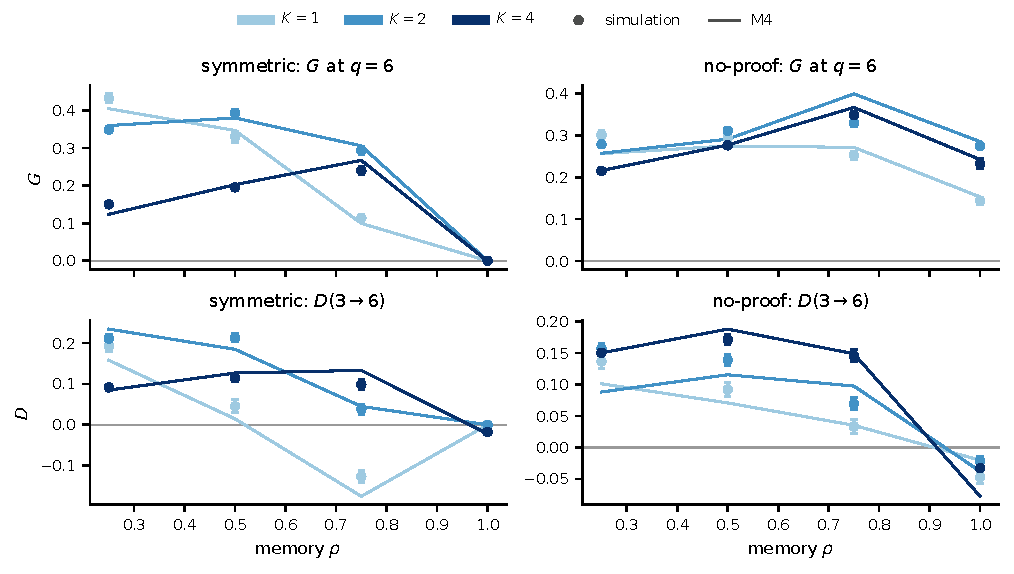
\includegraphics[width=\linewidth]{fig7_scaling_K.pdf}
\caption{\textbf{K independent projects} (simulation: 1{,}000 paired episodes for $K\le2$, 500 for $K=4$; M4: 40
realisations for $K=1$, 20 for $K=2,4$; post-hoc). The reversal survives at every $K$; its crossover moves to higher memory,
and M4 follows it.}
\label{fig:scaling}
\end{figure}
The reversal survives at $K=2$ and $4$ (Fig.~\ref{fig:scaling}), but its crossover moves to higher memory. At symmetric
$\rho=0.75$, $D(3\to6)$ goes from $-0.13$ ($K=1$) to $+0.04$ ($K=2$) and $+0.10$ ($K=4$). We had predicted, before the
data, that the results would not change with $K$, since copies per fact stay constant. That prediction was wrong. M4
follows the shift: $-0.17$, $+0.05$, $+0.13$; it gets 7/7, 7/7 and 8/8 resolved signs right with $G$ error 0.018,
0.019 and 0.013 for $K=1,2,4$ (M3: 5/7, 6/7, 6/8; 0.072, 0.031, 0.021).

\textbf{A confound.} A fact about one of $K$ projects is less informative about the summed answer: the range of $P(A2)$
over single facts shrinks from 0.21--0.45 ($K=1$) to 0.28--0.39 ($K=4$). In the no-proof worlds, the agents' pooled
evidence also leans toward $A2$ (0.42/0.58 at $K=2$, 0.37/0.63 at $K=4$). For a fixed decision, facts cannot multiply
while each stays as informative and the total evidence stays exactly sufficient. Copies per fact, informativeness per
fact and total evidence should be treated as separate parameters.

\subsection{Pre-registered test on a second task: Object Placements}
\label{sec:op}
\textbf{World.} MuSR~\cite{sprague2024musr} generates Object Placements stories from a symbolic skeleton: people move
items between locations, and each non-mover sees a move with some probability. We enumerated MuSR's generator exactly, for
3 people, 2 items, 3 locations (MuSR's most common number of answer options) and 3 moves, with a probability of $1/3$ that a
non-mover sees a move (MuSR uses 0.33). This gives 617{,}472 stories with their probabilities. The enumeration matches
frequencies sampled from MuSR's own code. Facts are abstract propositions:
\begin{itemize}
\item who moved what, and where;
\item who saw or missed each move;
\item what each person believes after each move, except the answer itself.
\end{itemize}
The chosen story has 34 true facts. The question is \emph{where would Casey look for the keys?} Its answers are
$A0=$ drawer (Casey's belief, correct), $A1=$ shelf, and $A2=$ desk (where the keys really are: the controller's target).

\textbf{Setups} follow task003's rules. Symmetric: 18 distinct agent facts jointly prove $A0$, and no single fact or pair
does. The controller's pool alone gives $P(A2)=0.98$ (task003: 0.89). No-proof: 15 agent facts leave exactly
$(0.5,0,0.5)$, and no single fact is more than 45\% sure. Two differences from task003: the no-proof pool alone favours
the truth, $(0.67,0,0.33)$, and the symmetric $A0$ pool reuses six agent facts, because the story has fewer true facts.

\begin{figure}[t]
\centering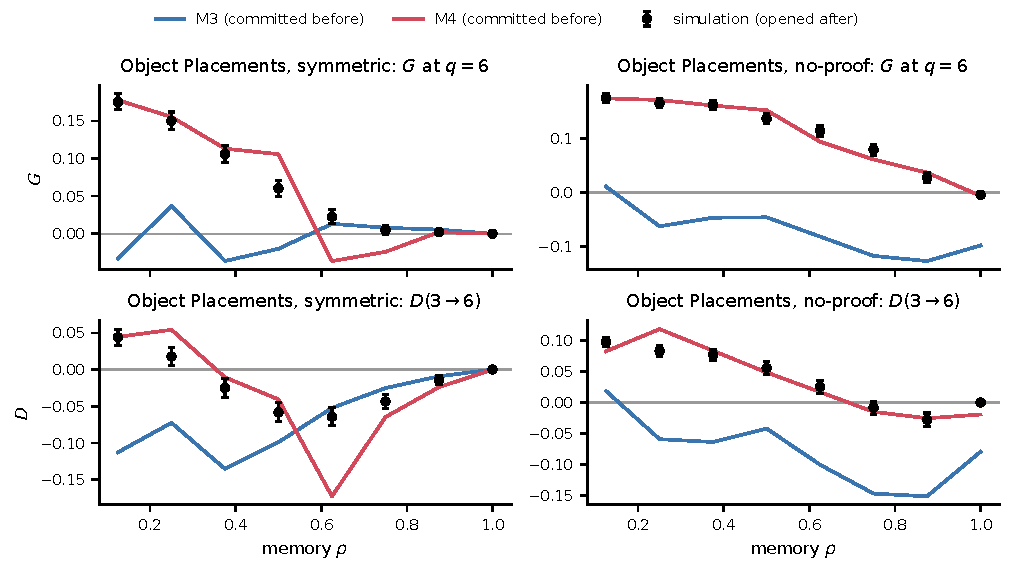
\includegraphics[width=\linewidth]{fig8_object_placements.pdf}
\caption{\textbf{Pre-registered test on Object Placements.} Lines: M3 and M4 predictions, committed before the
simulation data were opened. Points: simulation (1{,}000 paired episodes, 95\% intervals).}
\label{fig:op}
\end{figure}
\textbf{The reversal exists here too} (Fig.~\ref{fig:op}, Table~\ref{tab:opflips}). It shows the same qualitative
pattern: it appears in both setups, the no-proof setup reverses at higher memory, and the crossover falls with $q$. Two
things differ from task003: the symmetric crossover sits at lower memory, and the increments are about half as large.

\begin{table}[h]
\centering\small
\resizebox{\linewidth}{!}{%
\begin{tabular}{@{}llccc@{}}
\toprule
setup & step & Object Placements (simulation) & task003 (simulation) & Object Placements, M4 (pre-registered) \\
\midrule
symmetric & $3\to6$ & 0.25--0.375 & 0.5--0.625 & \textbf{0.25--0.375} \\
symmetric & $6\to9$ & 0.125--0.375 & 0.125--0.375 & 0.375--0.5 (and a spurious change) \\
no-proof  & $3\to6$ & 0.625--0.875 & 0.75--1 & 0.625--0.75 \\
no-proof  & $6\to9$ & 0.5--0.75 & 0.5--0.875 & 0.5--0.625 (and a spurious change) \\
\bottomrule
\end{tabular}}
\caption{Where the resolved sign of $D$ changes ($\rho$ bracket).}
\label{tab:opflips}
\end{table}

\textbf{Scores} (Table~\ref{tab:op}). M4's predictions get every resolved sign of $D(3\to6)$ right. Its error on $G$ is
0.030 (symmetric) and 0.019 (no-proof), and it predicts the symmetric crossover exactly. Its misses are small increments
of the later steps ($6\to9$, $9\to12$), whose size is comparable to M4's own sampling noise with 20 realisations. M4 also
overshoots the size of the symmetric $D(3\to6)$ at $\rho=0.625$ ($-0.17$ against $-0.06$; same sign). One
failure is not noise: at symmetric $\rho=0.5$--$0.75$, M4 predicts a small backfire ($G$ of $-0.04$ to $-0.02$ at
$\rho=0.625$--$0.75$) where the simulation shows a small positive effect. M3 fails. Its signs are 5/16 and 3/15, and it
predicts a backfire in no-proof ($G$ of $-0.05$ to $-0.13$) where the simulation shows positive effects up to $0.17$.

\begin{table}[h]
\centering\small
\resizebox{\linewidth}{!}{%
\begin{tabular}{@{}lccc@{}}
\toprule
 & resolved signs of $D$ (data $+$ / data $-$) & $G$ error & $3\to6$ crossover (simulation $\to$ model) \\
\midrule
M4, symmetric & 11/16 (3/3, 8/13) & \textbf{0.030} & 0.25--0.375 $\to$ \textbf{0.25--0.375} \\
M4, no-proof  & 12/15 (11/13, 1/2) & \textbf{0.019} & 0.625--0.875 $\to$ 0.625--0.75 \\
M3, symmetric & 5/16 (0/3, 5/13) & 0.066 & 0.25--0.375 $\to$ none \\
M3, no-proof  & 3/15 (1/13, 2/2) & 0.212 & 0.625--0.875 $\to$ 0.125--0.25 \\
\bottomrule
\end{tabular}}
\caption{Pre-registered scores on Object Placements (three reading steps, 8 values of $\rho$).}
\label{tab:op}
\end{table}

\subsection{Summary of all tests}
\begin{figure}[t]
\centering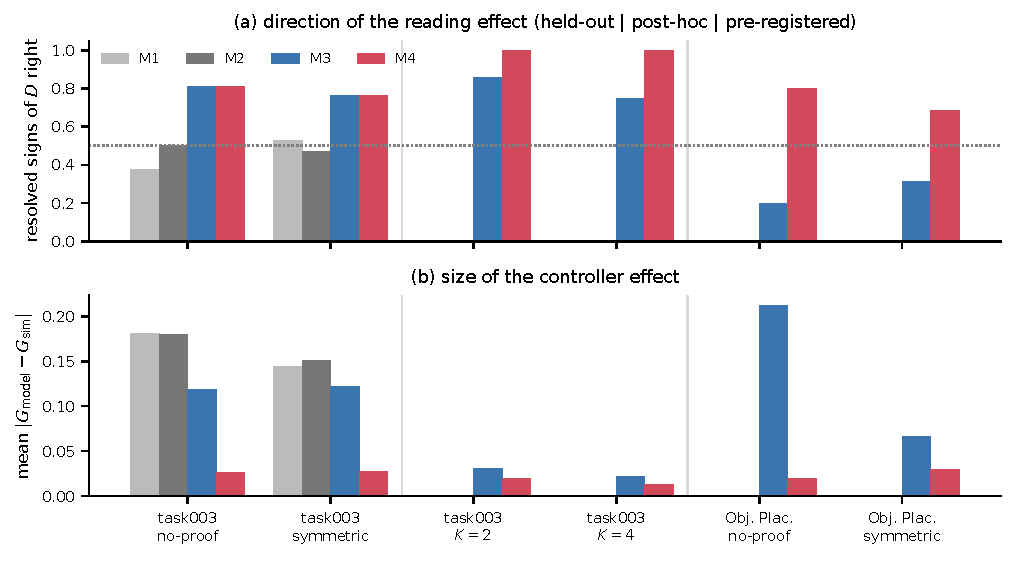
\includegraphics[width=\linewidth]{fig9_scoreboard.pdf}
\caption{\textbf{Every test in one place.} (a) Share of resolved reading increments whose sign the model gets right
(dotted: chance for a two-way call). (b) Mean absolute error of $G$. Groups: task003 held-out (pre-registered split),
K-projects (post-hoc), Object Placements (pre-registered predictions). M1 and M2 were not run beyond task003.}
\label{fig:scoreboard}
\end{figure}
Figure~\ref{fig:scoreboard} collects the tests. M4 is the only model whose error on $G$ stays at or below 0.03 in every
test. It also gets at least 69\% of resolved signs right in every test.

% ======================================================================================================================
\section{Discussion}
\label{sec:discussion}
\paragraph{What the evidence supports.} The controller's power and its persistence come from a finite-swarm property:
facts are held by about one agent each, they go extinct, and extinction is permanent. Deterministic theories miss this
by construction. The two models that contain it, M3 and M4, recover the signs, and the one that also lets every reader see
the same fluctuating board (M4) recovers the magnitudes. That held on held-out data, on a scaling family it was not
built for, and on a second task, before its data were seen.

\paragraph{Why reading can help or hurt.} Eq.~\eqref{eq:Rf} shows that reading raises the reproduction of every fact.
Whether this helps the controller depends on whose facts are near the extinction threshold. With fast forgetting, agent
facts die anyway, and more reading mainly spreads the controller's facts. With slow forgetting, more reading rescues the
swarm's own evidence. The crossover then depends on how much evidence the swarm needs (a proof in the symmetric setup,
less in the no-proof setup) and on how informative each fact is, which is why it moves between tasks and with $K$.

\paragraph{Limitations.}
\begin{itemize}
\item M4 is a reduced stochastic model. We have no closed-form result, such as an extinction probability of a fact as a
  function of $(\rho,q)$ or a condition for the sign of $D$.
\item The held-out task003 data had been seen in earlier descriptive reports.
\item M4's predictions near $D=0$ carry sampling noise (20--40 realisations), so sign errors at crossovers may partly be
  model noise.
\item The K-projects family changes how informative each fact is along with the number of facts.
\item Persistence was tested only on task003.
\item Shared approximations of all models: a reader's own posts are not excluded from its window, the time step is
  $dt=0.05$, and the controller in M1--M3 is an expected controller.
\end{itemize}

\paragraph{Next steps.}
\begin{itemize}
\item An analytical treatment of fact extinction, for example a branching-process approximation with per-fact rates
  taken from Eq.~\eqref{eq:Rf}~\cite{harris1963}, or a Moran-type neutral-drift account of
  persistence~\cite{moran1958,ewens2004}.
\item A scaling family that varies copies per fact, informativeness and total evidence one at a time.
\item Persistence experiments on Object Placements.
\item Interventions the theory suggests, such as deduplicated reading, which lowers the controller's reproduction
  advantage.
\item A transfer test with language-model agents.
\end{itemize}

\paragraph{Related work.} Statistical physics of opinion and social dynamics~\cite{castellano2009} studies consensus
in agent populations, usually with agents that copy opinions rather than reason from evidence. Our agents are exact
Bayesian reasoners, and the quantities that drift are facts, not opinions. Fact counts behave like allele counts in
finite populations~\cite{moran1958,ewens2004}, and the failure of deterministic closures for rare types is the classical
reason for stochastic treatments~\cite{vankampen1992}.

\paragraph{Reproducibility.} Code, data tables and scorecards are in the project repository. Paths are relative
to its \nolinkurl{analysis/} folder:
\begin{itemize}
\item simulator: \nolinkurl{task003_llm_free/simulation_2/simulator/};
\item models M1--M4: \nolinkurl{theory/models/mean_field.py};
\item model runner: \nolinkurl{theory/models/run_models.py};
\item split and scorecards: \nolinkurl{task003_llm_free/simulation_2/key_phenomena_hypothesis/};
\item Object Placements: \nolinkurl{object_placements_llm_free/};
\item figures of this report: \nolinkurl{theory/reports/2026-10-23_theory_report/make_figures.py}.
\end{itemize}

\begin{thebibliography}{9}\small
\bibitem{sprague2024musr} Z.~Sprague, X.~Ye, K.~Bostrom, S.~Chaudhuri, G.~Durrett. MuSR: Testing the limits of
chain-of-thought with multistep soft reasoning. \emph{ICLR}, 2024. arXiv:2310.16049.
\bibitem{vankampen1992} N.~G.~van Kampen. \emph{Stochastic Processes in Physics and Chemistry}. North-Holland, 1992.
\bibitem{harris1963} T.~E.~Harris. \emph{The Theory of Branching Processes}. Springer, 1963.
\bibitem{moran1958} P.~A.~P.~Moran. Random processes in genetics. \emph{Mathematical Proceedings of the Cambridge
Philosophical Society} 54:60--71, 1958.
\bibitem{ewens2004} W.~J.~Ewens. \emph{Mathematical Population Genetics I: Theoretical Introduction}. Springer, 2nd ed., 2004.
\bibitem{castellano2009} C.~Castellano, S.~Fortunato, V.~Loreto. Statistical physics of social dynamics. \emph{Reviews of
Modern Physics} 81:591--646, 2009.
\end{thebibliography}

\end{document}
